%!TEX root = ../thesis.tex

\chapter{Eigener Ansatz} % (fold)
\label{cha:eigener_ansatz}


\begin{itemize}
    \item Probleme und deren Lösung während der Umsetzung
    \item Beispiel: Zugriff auf Moodle über Webservice
\end{itemize}

\section{Datenformat} % (fold)
\label{sec:datenformat}

% section datenformat (end)

\section{Social Online Community Connectors} % (fold)
\label{sec:social_online_community_connectors}

\subsection{Konfiguration} % (fold)
\label{sub:konfiguration}

Eine wichtige Designentscheidung der Connectoren war es, wo alle zum Betrieb notwendigen Einstellungen und zusätzliche Daten gespeichert werden sollen? In den ersten Testimplementierungen wurden diese Daten teilweise in einfachen Dateien, nur für die anfallenden Daten im RDF Format war von Beginn an eine Speicherung in einem RDF Triplestore vorgesehen. Im späteren Verlauf dieser Arbeit kam die Idee auf komplett alle Daten dort zu speichern. Da es vorkommen kann, dass bestimmte Einstellungen wie Anmeldedaten mehrfach genutzt werden und im Falle eine Änderung müssten die Daten nur an diesem einen Ort geändert werten. So könnten auch diverse Einstellungen über verschiedene unabhängige System hinweg genutzt werden. 

\medskip

Aus diesem Grunde wurde für die Konfiguration eines Connectors die \emph{Connector Config Ontology} entwickelt. Abbildung \ref{fig:uebersicht_conector_cfg} zeigt diese Ontologie. Jeder Connector bekommt einen eindeutigen Bezeichner(kurz ID) um jeden diesen identifizieren zu können. Dies kann eine beliebige Zeichenkette sein. Um die korrekte Javaklasse des zu erstellenden Connectors benutzen zu können, wird der vollständige Klassenname, wie er zum Beispiel von \lstinline{object.class.getName()} zurückgegeben wird, in \texttt{connectorClassName} gespeichert. Für den Zugriff auf die Daten der SOC sind bei einiges APIs bestimmte Parameter wie die genaue Adresse des Servers notwendig. SIOC bietet hierzu ein eigenes Modul an was genau für solche Beschreibungen die SIOC Ontologie erweitere. Eine kurze Beschreibung dieses Moduls und eine Erweiterung für den Einsatz in SOCC befindet sich im Abschnitt \ref{ssub:services} und \ref{ssub:authorization}. Als Letztes braucht ein Connector noch einen vordefinierten Benutzer welcher als \texttt{defaultUserAccount} als SIOC UserAccount gespeichert wird. Dieser vordefinierte erfüllt im Großen und Ganzen zwei Aufgaben. Als Erstes wird er für lesende Zugriffe der API auf die SOC genutzt, da hierzu ein einzelner Benutzer vollkommen ausreichend ist. Die zweite Aufgabe bezieht sich auf das stellvertretende Schreiben einzelner Benutzer. Nicht immer werden die dazu notwendigen Daten von den Benutzer zur Verfügung gestellt oder sind unbekannt. In diesem Fall wird der vordefinierte Benutzer genutzt und der Beitrag mit einem Vermerk zum original Autor über diesen geschrieben.

\begin{figure}[ht]
    \centering
    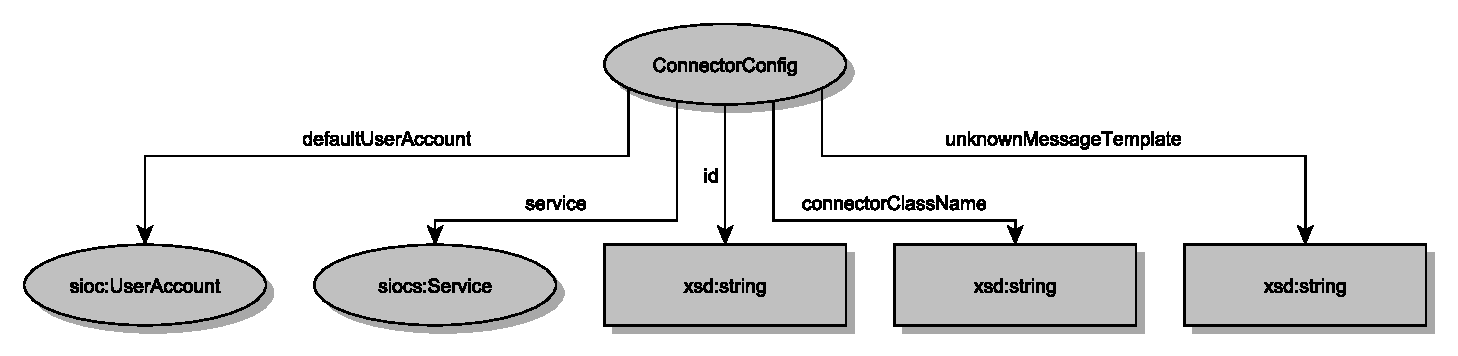
\includegraphics[
        width=\textwidth,
        keepaspectratio=true
    ]{assets/images/connector_config_ontology}
    \caption{Connector Config Ontology}
    \label{fig:uebersicht_conector_cfg}
\end{figure}

\subsubsection{Services} % (fold)
\label{ssub:services}

% subsubsection services (end)

\subsubsection{UserAccounts} % (fold)
\label{ssub:useraccounts}

% subsubsection useraccounts (end)

\subsubsection{Autorisierung} % (fold)
\label{ssub:authorization}

% subsubsection authorization (end)

% subsection konfiguration (end)

\subsection{Aufbau} % (fold)
\label{sub:aufbau}

\begin{figure}[ht]
    \centering
    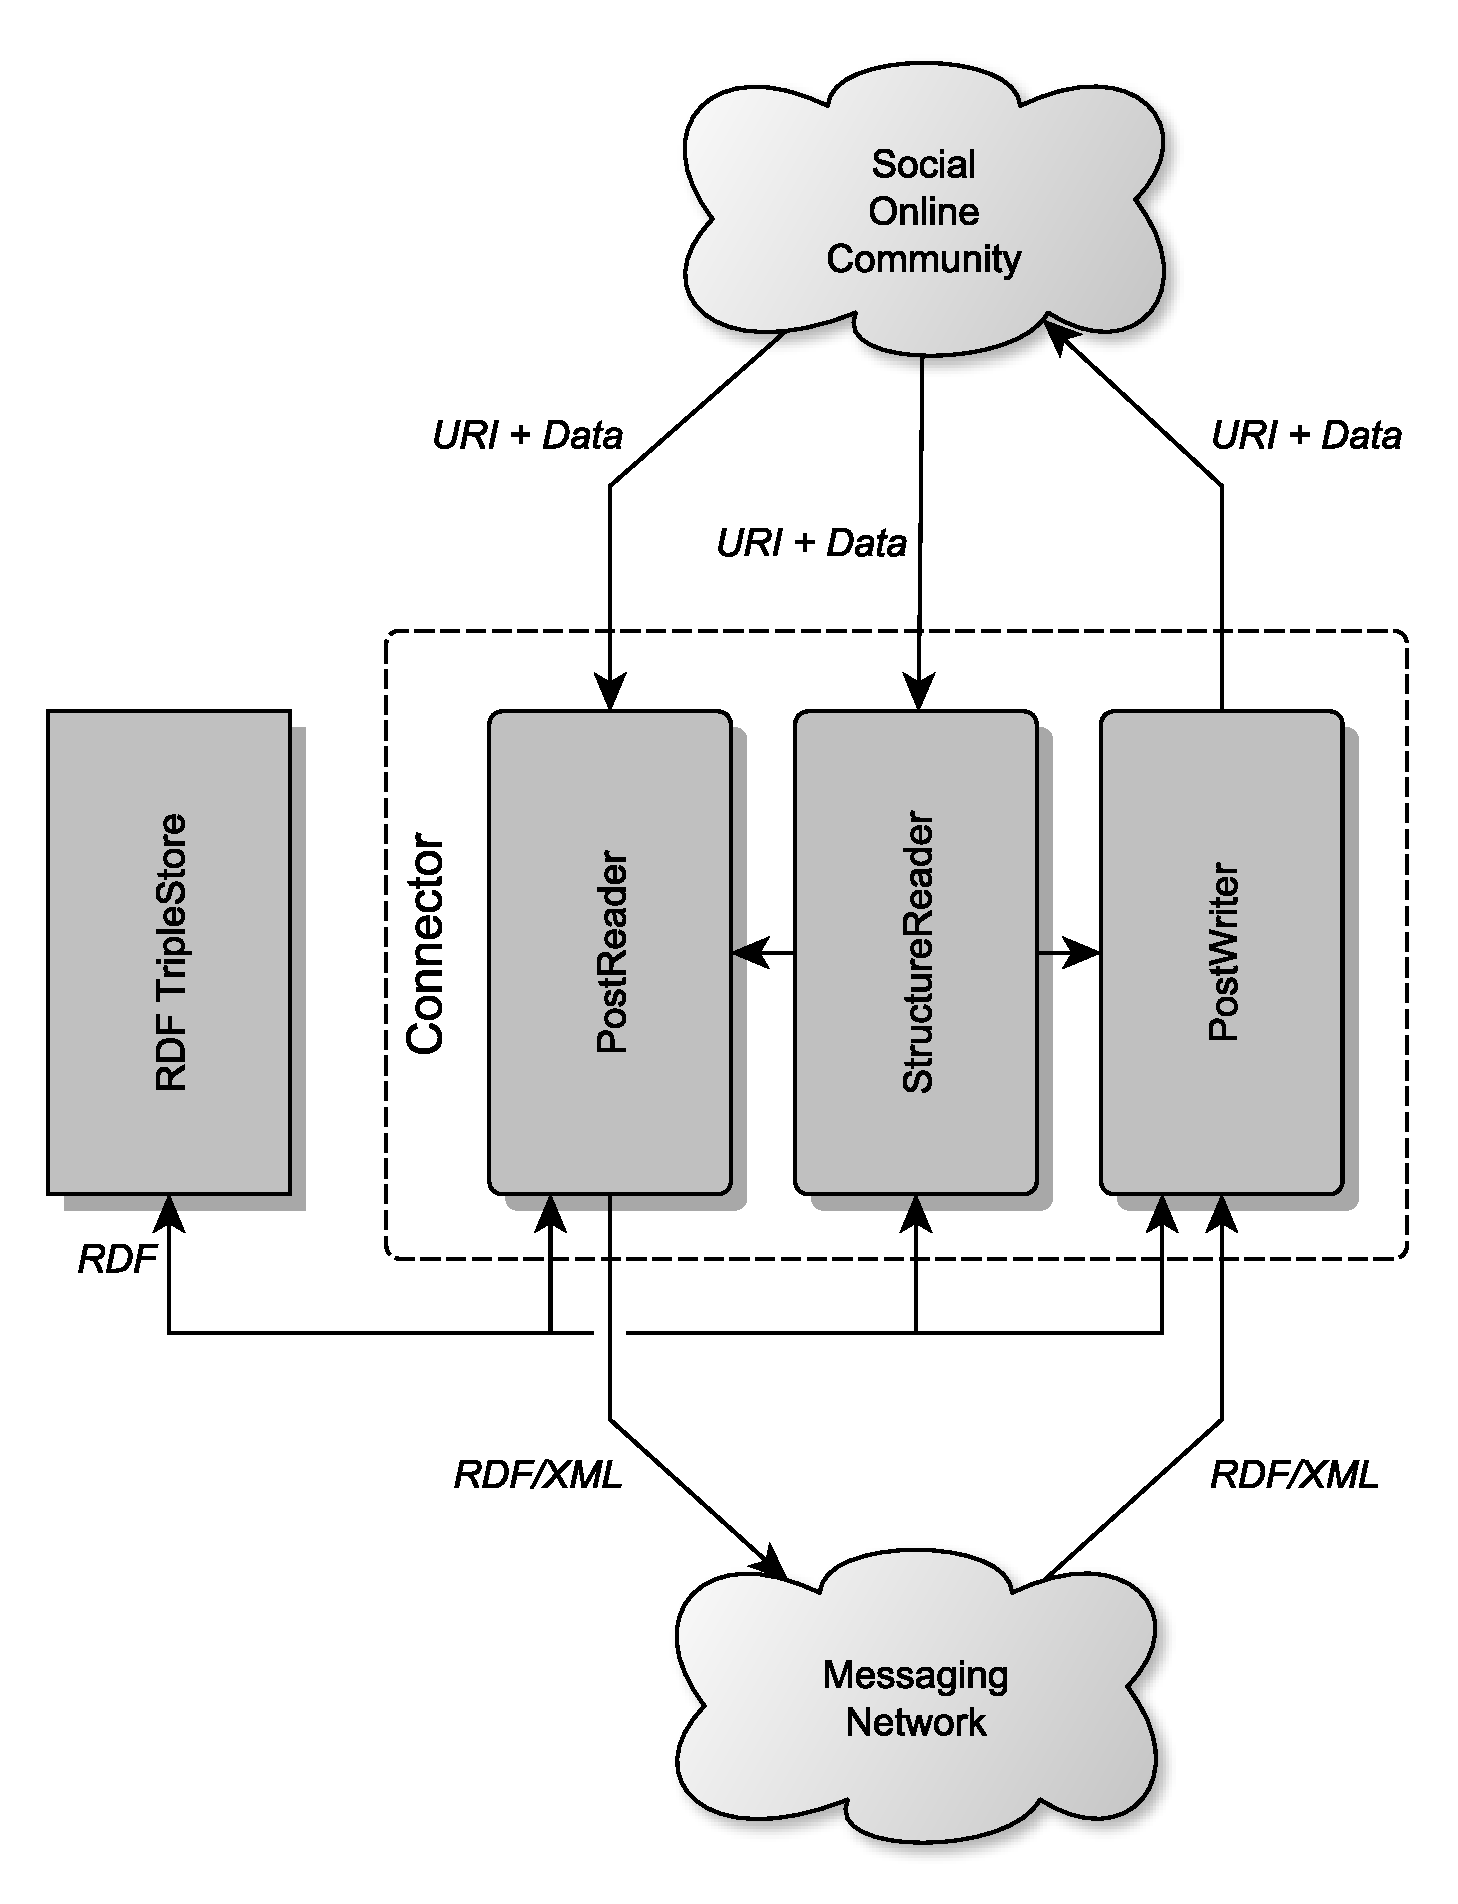
\includegraphics[
        width=0.5\textwidth,
        keepaspectratio=true
    ]{assets/images/socc_connector_overview.pdf}
    \caption{Übersicht der Komponenten der SOCC}
    \label{fig:uebersicht_socc}
\end{figure}

\subsubsection{ClientManager} % (fold)
\label{ssub:clientmanager}

% subsubsection clientmanager (end)

\subsubsection{StructureReader} % (fold)
\label{ssub:structurereader}

\begin{wrapfigure}[10]{r}{7cm}
    \centering
    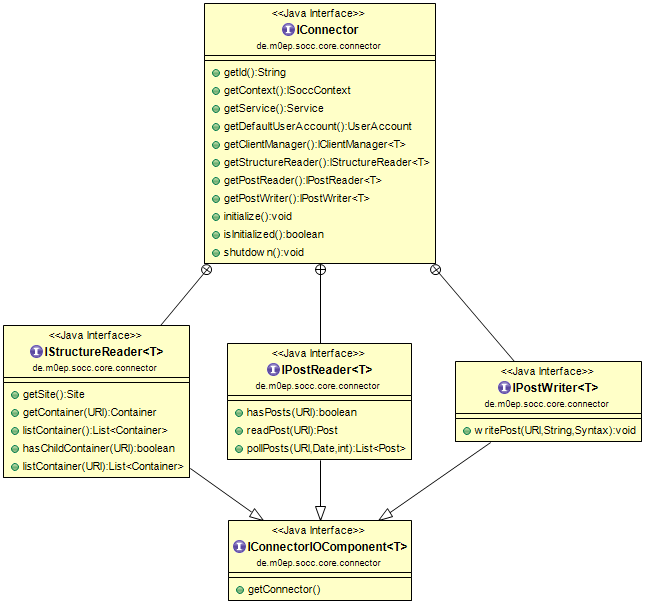
\includegraphics[
        width=5cm,
        keepaspectratio=true,
        clip=true,
        trim= 0 126 456 326
    ]
    {assets/images/uml_iconnector.png}
    \caption{StructurReader}
    \label{fig:uml_structure_reader}
\end{wrapfigure}
Um auf Informationen über die Struktur von Foren, sozialen Netzwerken und so weiter im SIOC Format zugreifen zu können, implementiert jeder Connector dazu einen StructureReader. Die Struktur lässt sich, wie im Abschnitt \ref{sec:social_online_community_connectors} gezeigt, durch die SIOC Klassen \emph{Site} und \emph{Container} (und Unterklassen davon) beschrieben. Um auf diese Struktur zugreifen zu können, enthält die StructureReader Schnittstelle mehrere Methode (Siehe Abbildung \ref{fig:uml_structure_reader}). \wrapfill

\begin{description}
    \item[\texttt{getSite()}] ist eine Methode, welche die Beschreibung einer Seite (Forum, Blog, soziales Netzwerk) als SIOC Site Objekt zurücklieft. Dies wird relativ häufig um die Zugehörigkeit einiger Objekte durch einen Link zu dieser Seite zu verdeutlichen. Dies kann bei einigen APIs nützlich sein, da dort manchmal keine Information zum \emph{Container} eines Beitrags mitgeliefert werden, über den man sonst eine Beziehung zwischen Seite und Beitrag herstellen könnte.

    \item[\texttt{getContainer(URI)}] ist dazu gedacht die Information eines einzelnen Containers erhalten der sich hinter eine URI verbirgt.

    \item[\texttt{listContainer(...)}] sind Methoden welche für den die Auflisten aller Container einer Seite zur Verfügung stehen. Die Methode ohne Parameter listet alle Container auf der ersten Ebene auf. Dies könnten zum Beispiel alle Kurse auf einen Canvas LMS Seite oder alle Gruppen auf Facebook sein. Die zweite Methode mit URI Parameter gibt eine Liste alle Container, welche den Container hinter der übergeben URI als Elternteil haben, zurück. Als Beispiel wären alle Themen innerhalb eines Forums zu nennen.

    \item[\texttt{hasChildContainer(URI)}] überprüft ob der Container hinter einer URI überhaupt weitere Container als Kinder besitzt. Diese Methode wird dazu eingesetzt, um vorab zu testen, ob der Aufruf von \texttt{listContainer(URI)} das gewünschte Ergebnis liefert oder ein Fehler auftritt. 
\end{description}


% subsubsection structurereader (end)

\subsubsection{PostReader} % (fold)
\label{ssub:postreader}

\begin{wrapfigure}{r}{7cm}
\centering
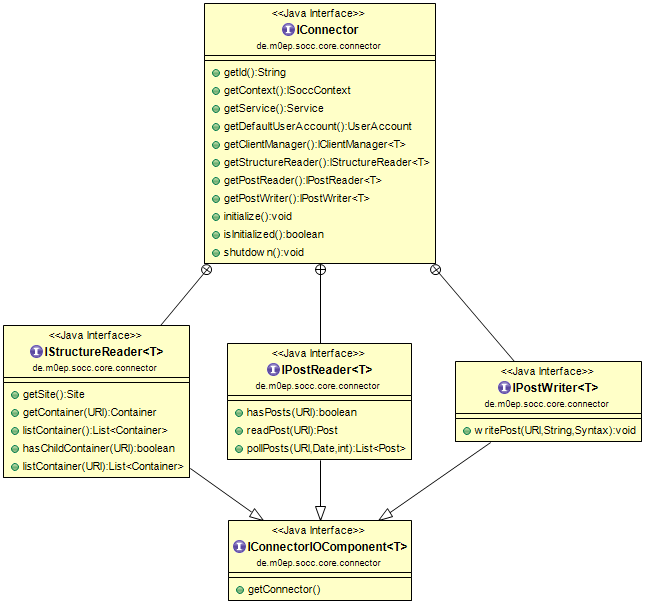
\includegraphics[
width=6cm,
keepaspectratio=true,
clip=true,
trim= 220 144 220 344
]{assets/images/uml_iconnector.png}
\caption{PostReader}
\end{wrapfigure}

Der \texttt{PostReader} dient als Schnittstelle, um auf geschriebene Beitrage innerhalb eines Containers oder die Kommentare auf eines Beitrags zuzugreifen. Die Methode \texttt{hasPosts(URI)} ist nur zur Überprüfung ob ein Container oder ein Beitrag hinter einer URI weiter Beiträge enthält die gelesen werden können. Um einen einzelnen Beitrag anhand seiner URI lesen zu können kann die Methode \texttt{getPost(URI)}  genutzt werden. Sei liefert dann den Beitrag SIOC Post Objekt zurück beziehungsweise einen Fehler, falls der Beitrag nicht mit diesem Connector gelesen werden kann. Die wichtigste Methode dahingegen ist \texttt{pollPosts(URI, Date, int)}. Insgesamt können dieser Methode drei Parameter übergeben werden. Der Erste ist eine URI die den Ort angibt von der alle Beiträge gelesen werden können. Mit dem zweiten Parameter kann ein Zeitpunkt angegeben werden, ab dem ein zu lesender Beitrag geschrieben sein muss. Alle Beiträge die vor diesem Zeitpunkt erstellt wurden, werden nicht zurück gegeben. Der letzte Parameter gibt eine obere Schranke an wie viele Beiträge maximal pro Aufruf dieser Methode gelesen werden dürfen.

% subsubsection postreader (end)

\subsubsection{PostWriter} % (fold)
\label{ssub:postwriter}

In Abbildung \ref{fig:postwriter_sequenzdiagramm} ist ein Sequenzdiagramm der PostWriter Komponente zu sehen. Dort ist visualisiert, welche Schritte für das stellvertretende Schreiben von Beiträgen eines Benutzers unternommen werden müssen. Soll nun ein Beitrag in einer SOC geschrieben werden, wird die Methode \texttt{writePost(URI, String, Syntax)} mit dem Zielort als URI, dem Beitrag als serialisiertes RDF Objekt und dem verwendeten Serialisierungsformates aufgerufen. Begonnen wird damit, dass als erstes nach einem UserAccount für den Service des aktuellen Connectors des Beitragautors gesucht. Im Idealfall befindet sich für den UserAccount des Beitragsautors ein Link zu seiner FOAF Person und von ein weiterer Link zum UserAccount für den aktuellen Service. Mit diesem UserAccount kann dann vom ClientManager ein Clientobjekt für die verwendete API angefordert werden. Sollte die Suche negativ verlaufen, steht der vordefinierte Client zur Verfügung. Mit diesem Client, ob mit der des Autors oder dem Vordefinierten, wird im letzten Schritt der Beitrag im von der API verwendeten Format in die SOC geschrieben.
\begin{figure}[h]
\centering
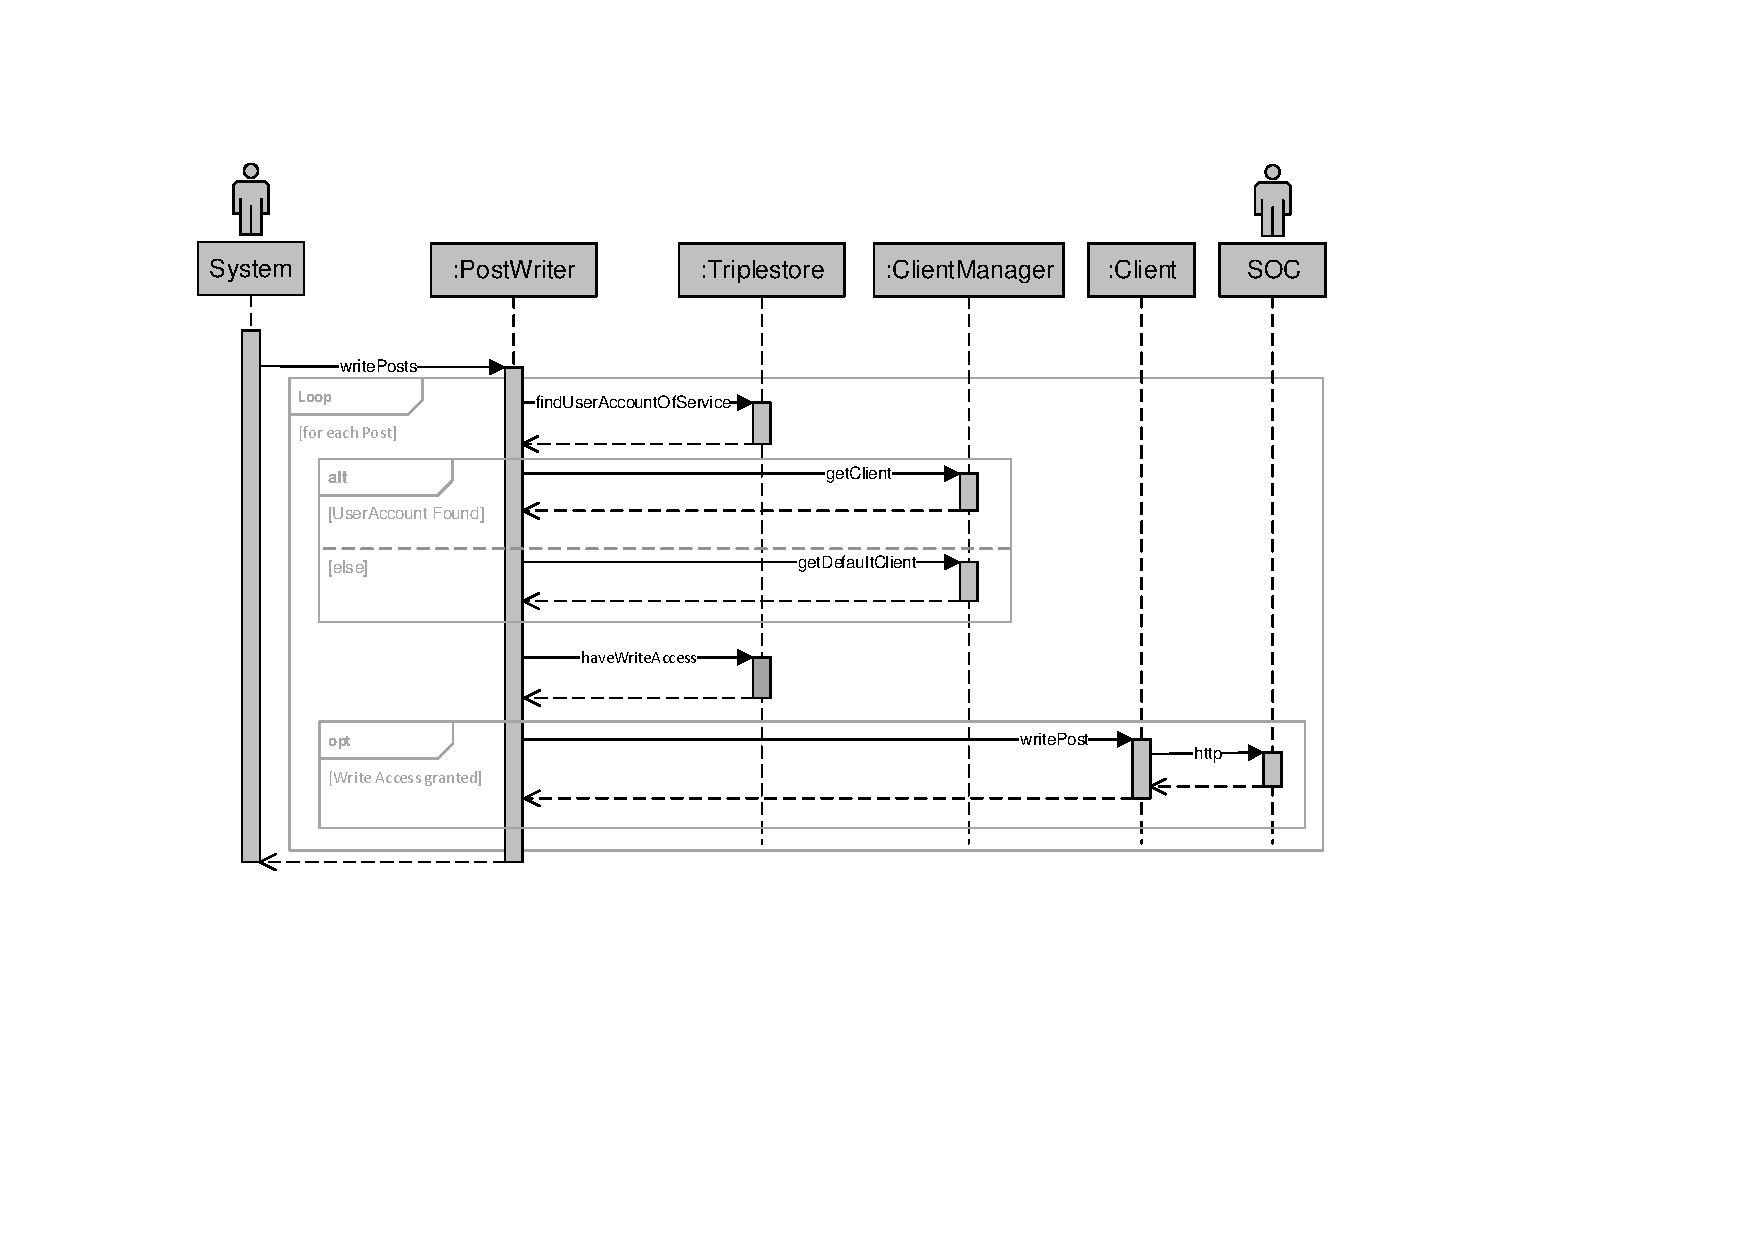
\includegraphics[
width=\textwidth,
keepaspectratio=true,
clip=true,
trim= 90 200 220 75
]{assets/images/postwriter_sequencediagram}
\caption{PostWriter Sequenzdiagramm}
\label{fig:postwriter_sequenzdiagramm}
\end{figure}

% subsubsection postwriter (end)

% subsection aufbau (end)

\subsection{Moodle Connector} % (fold)
\label{sub:moodle_connector}

% subsection moodle_connector (end)

\subsection{Facebook Connector} % (fold)
\label{sub:facebook_connector}

% subsection facebook_connector (end)

\subsection{Google+ Connector} % (fold)
\label{sub:google_plus_connector}

% subsection google_connector (end)

\subsection{Youtube Connector} % (fold)
\label{sub:youtube_connector}

% subsection youtube_connector (end)

\subsection{Canvas LMS Connector} % (fold)
\label{sub:canvas_lms_connector}

% subsection canvas_lms (end)

% section social_online_community_connectors (end)

\section{SOCC-Camel} % (fold)
\label{sec:socc_camel}

\begin{figure}[ht]
     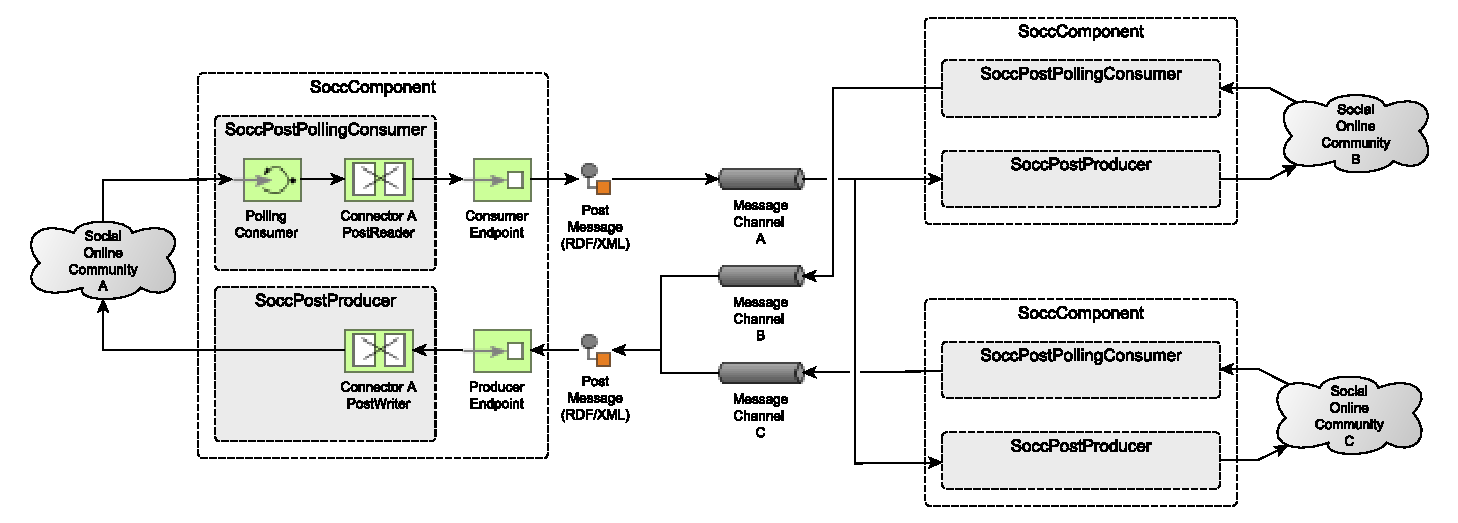
\includegraphics[
        width=\textwidth,
        keepaspectratio=true
    ]{assets/images/socc_camel_overview}
    \caption{Übersicht des Apache Camel Moduls Socc-Camel}
    \label{fig:uebersicht_socc_camel}
\end{figure}

\subsection{SoccComponent} % (fold)
\label{sub:socccomponent}

% subsection socccomponent (end)

\subsection{SoccPostPollingConsumer} % (fold)
\label{sub:soccpostpollingconsumer}

% subsection soccpostpollingconsumer (end)

\subsection{SoccPostProducer} % (fold)
\label{sub:soccpostproducer}

% subsection soccpostproducer (end)

% section socc_camel (end)

% chapter eigener_ansatz (end)
